\documentclass[tikz,border=2pt]{standalone}
\usepackage{amsmath,amssymb}
\usepackage{tikz}

\begin{document}
% x_i -> x: for any ball around x, all terms from some index N on lie inside it.
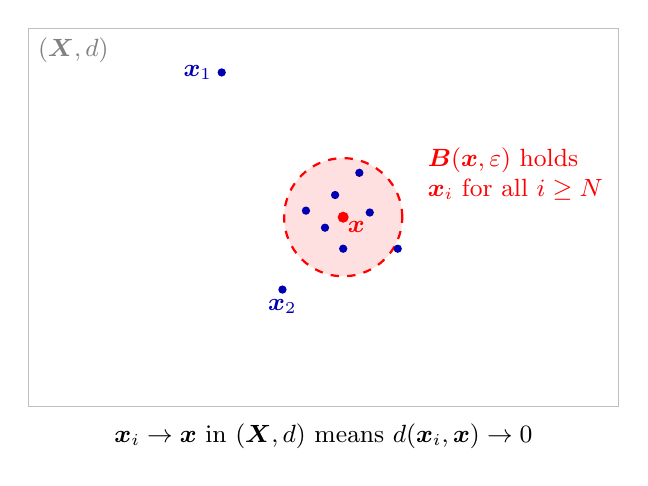
\begin{tikzpicture}[every node/.style={font=\small}]
	\draw[gray!50] (-3.2,-2.2) rectangle (4.3,2.6);
	\node[gray, anchor=north west] at (-3.2,2.6) {$(\boldsymbol{X},d)$};
	\fill[red!12] (0.8,0.2) circle (0.75);
	\draw[red, thick, dashed] (0.8,0.2) circle (0.75);
	\fill[red] (0.8,0.2) circle (2pt) node[below right, inner sep=1.5pt] {$\boldsymbol{x}$};
	\foreach \i in {1,...,9} {
		\pgfmathsetmacro{\r}{2.4/\i}
		\pgfmathsetmacro{\a}{100*\i+30}
		\fill[blue!70!black] ({0.8+\r*cos(\a)},{0.2+\r*sin(\a)}) circle (1.5pt);
	}
	\node[blue!70!black, anchor=east] at ({0.8+2.4*cos(130)},{0.2+2.4*sin(130)}) {$\boldsymbol{x}_1$};
	\node[blue!70!black, anchor=north] at ({0.8+1.2*cos(230)},{0.2+1.2*sin(230)}) {$\boldsymbol{x}_2$};
	\node[red, anchor=west, align=left] at (1.75,0.75) {$\boldsymbol{B}(\boldsymbol{x},\varepsilon)$ holds\\ $\boldsymbol{x}_i$ for all $i\ge N$};
	\node[anchor=north] at (0.55,-2.3) {$\boldsymbol{x}_i\to\boldsymbol{x}$ in $(\boldsymbol{X},d)$ means $d(\boldsymbol{x}_i,\boldsymbol{x})\to 0$};
\end{tikzpicture}
\end{document}
